\chapter{Introduzione}
In questo capitolo verrà descritto in modo più approfondito il funzionamento della piattaforma Moon Cloud e unitamente al 
motivo dell'implementazione della soluzione proposta.

\section{MoonCloud overview}
La diffusione di sistemi ICT (\textit{Information and Communications Technology}) nella maggiorparte degli ambienti lavorativi 
e privati in termini di servizi offerti, automazione di processi e incremento delle performance. L'uso di questa tecnologia 
ha assunto importanza a partire dagli anni novanta come effetto del boom di Internet.
Oggi le professionalità legate all'ICT crescono in numero e si evolvono per specificità, per operare in ambienti fortemente 
eterogenei ma sempre più interconnessi fra di loro come il cloud computing, i social newtwork, il marketing digitale, i sistemi IoT, 
la realtà virtuale, etc.

Gli immensi benefici del cloud in termini di flessibilità, consumo delle risorse e gestione semplificata, la rende la prima 
scelta per utenti e industrie per il deploy dei loro sistemi IT. Tuttavia il cloud computing solleva diverse problematiche
legate alla mancanza di fiducia e trasparenza dove i clienti necessitano di avere delle garanzie sui servizi cloud ai quali 
si affidano; spesso i fornitori di servizi cloud non fornisco ai clienti le specifiche riguardanti le misure di sicurezza 
messe in atto.

Negli ultimi anni, sono state sviluppate tecniche e modi per rendere sicuri questi sistemi e proteggere i dati degli utenti, 
portando alla diffusione di approcci eterogenei che incrementaro la confusione negli utenti.
Tecniche tradizionali di verifica della sicurezza basati su approcci di analisi statistica non sono più sufficenti e
devono essere integrati con processi di raccolta di evidence da sistemi cloud in produzione e funzionamento. 
In generale il \textit{cloud security} definisce i modi (ad esempio criptazione, controllo degli accessi, etc.) per 
proteggere attivamente gli asset da minaccie interne ed esterne, e fornire un ambiente in cui i clienti possano affidarsi 
e interagire in totale sicurezza. 
Ma per rendere il cloud degno di fiducia e trasparente, sono state introdotte tecniche di \textit{security assurance} le 
quali sono definite come il modo per ottenere la fiducia necessaria nelle infrastrutture e/o nelle applicazioni di 
dimostrare che siano garantite delle proprietà di sicurezza, e che operi normalmente anche se subisce attacchi; grazie alla 
raccolta e allo studio di queste evidence è possibile che venga accertata la validità e efficenza delle proprietà di sicurezza.

Il prezzo che paghiamo per i benefici di queste tecnologie è dato dall'incremento di violazioni di sicurezza, che oggigiorno 
preoccupa tutte le aziende e anche i loro clienti, con l'incremento del rischio di fallimento per i servizi più importanti dovuti a
violazioni della privacy e al furto di dati.
\newline
Il mercato sta lentamente notando che non è l'inadequamento tecnologico dei sistemi di sicurezza che incrementa il rischio di furti 
di dati o delle violazioni di sicurezza; piuttosto, la mal configurazione e l'errata integrazione di questi sistemi nei processi 
di business. \cite{cloud-Platform-for-ICT-Security-Governance}

Per questo motivo anche se vengono usati i sistemi di sicurezza e di controllo migliori non è possibile garantire la sicurezza; 
ma è necessario implementare un processo continuo di diagnostica che verifica che i controlli siano configurati in modo corretto 
e il loro comportamento sia quello aspettato.

Il \textit{Security Assesment} diventa allora un aspetto importante specialmente negli ambienti cloud e IoT. Questo processo
deve essere portato avanti in modo continuo e olistico, per correlare le evidence raccolte da sempre maggiori meccanismi di 
protezione. \cite{mooncloud-semi-automatic-and-trustworthy}
\newline
Moon Cloud è una soluzione PaaS (Platform as a Service) che fornice una piattaforma B2B (Business To Business) innovativa per verifiche, 
diagnostiche e monitoraggio dell'adeguatezza dei sistemi ICT rispetto alle politiche di sicurezza, in modo continuo e su larga scala.
Moon Cloud supporta una semplice ed efficente \textit{ICT security governance}, dove le politiche di sicurezza possono
essere definite dalle compagnie stesse (a partire da un semplice controllo sulle vulnerabilità a linee guida di
sicurezza interna), da entità esterne, imposte da standard oppure da regolamentazioni nazionali/internazionali.
\newline
La sicurezza di un sistema o di un insieme di asset dipende solo parzialmente dalla forza dei singoli meccanismi di protezione isolati
l'uno dall'altro; infatti, dipende anche dall'abilità di questi meccanismi di lavorare continuamente in sinergia per provvedere a
una protezione olistica.
In più, quando i sistemi cloud e i servizi IoT sono coinvolti, le dinamiche di questi servizi e la loro rapida evoluzione rende il 
controllo dei processi all'interno dell'azienda e le politiche di sicurezza più complesse e prone ad errori.
\newline
I requisiti ad alto livello fondamentali per poter garantire le Security Assurance sono:
\begin{description}
	\item[sistema olistico] è richiesta una visione globale e pulita dello stautus dei sistemi di sicurezza; inoltre è cruciale 
	distribuire lo sforzo degli specialisti in sicurezza per migliorare il processo e le politiche messe in atto. Si parte da 
	delle valutazioni fatte manualmente a quella semi-automatiche che ispezionano i meccanismi di sicurezza. 
	\item[monitoraggio continuo ed efficiente] è necessario un controllo continuo che valuti l'efficenza dei sistemi di sicurezza 
	per ridurre l'impatto dell'errore umano, soprattutto dal punto di vista organizzativo. La mancata configurazione dovuta al 
	cambiamento dell'ambiente, la coesistenza di componenenti in conflitto: sono scenari che richiedono un monitoraggio e un 
	aggiornamento continuo.
	\item[singolo punto managment] avere un solo punto in cui gestire tutti gli aspetti relativi alla sicurezza, permette di avere 
	sotto controllo le politiche di sicurezza. Inoltre disporre di un inventario degli asset da proteggere, così da poter conoscere 
	quali protezioni applicare.
	\item[reazioni rapide a incidenti di sicurezza] spesso la reazione ad incidenti di sicurezza è ritardata da due fattori: il tempo 
	richiesto per rilevare l'incidente e il tempo per analizzare il motivo dell'accaduto.
\end{description}


Moon Cloud è basato su una tecnica di Security Assurance garantendo che tutte le attività aziendali si compiano seguendo i requisiti 
prestabiliti da appropriate politiche e procedure.

Una \textit{Security Compliance Evaluation} è il processo di verifica a cui un target viene sottoposto e il cui risultato deve 
soddisfare i requisiti richiesti da standard e politiche. A partire da questi processi di verifica, che devono a loro volta essere 
affidabili, si ottendo delle evidence; queste ultime possono essere raccolte monitorando l'attività del target oppure, come già 
menzionato, sottoponendo il target a scenari critici o di testing.
In particolare, una Security Compliance Evaluation è un processo che verifica l'uniformità di un certo target a una o più politiche 
attraverso una serie di controlli che a seconda dvalore booleano associato ad ogni controllo viene prodotto un valore booleano 
per le politiche.
\begin{figure}
	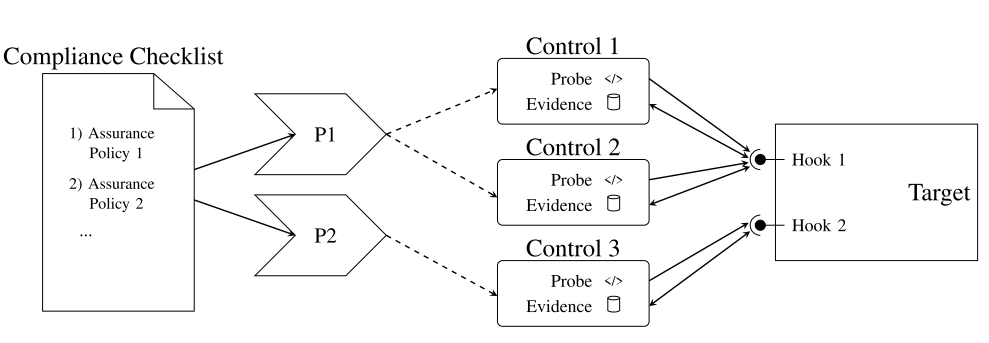
\includegraphics[scale=0.5]{images/Security_Compliance_Evaluation.PNG}
	\caption{Security Compliance Evaluation}
	\label{fig:Security_Compliance_Evaluation}
\end{figure}

\newpage

\section{Processo di Evaluation}
Moon Cloud implementa il processo di Security Compliance Evaluation in Figura \ref{fig:Security_Compliance_Evaluation} usando controlli 
di monitoraggio o di test personalizzabile. Inoltre garantisce, oltre a tutti i requisisti ad alto livello elencati prima, 
anche i seguenti:
\begin{description}
	\item Moon Cloud è una piattaforma cloud centralizzata presentando una visione olistica dello stato di sicurezza di un dato sistema.
	\item Moon Cloud implementa un sistema di Assurance Evidence-based continuo, implementato come processo di Compliance,
	basato su politiche custom o standard.
	\item Moon Cloud è offerto come un servizio - PaaS, dove le attività di evaluation possono essere facilmente ed efficentemente 
	configurate su un target asset, senza l'intervento dell'uomo.
	\item Moon Cloud permette di schedulare delle ispezioni automatiche, grazie all'inventario di asset protetto.
	\item Moon Cloud evaluation engine può ispezionare dall'interno, gestendo così delle minaccie interne; permettendo anche reazioni 
	rapide a incidenti di sicurezza e veloci rimedi, grazie alla raccolta continua di evidence. 
\end{description}


L'architettura di Moon Cloud è costituita da un'Assurance Manager che gestisce i processi di Evaluation attraverso un set di 
\textit{Execution Cluster}; ognuno dei quali gestisce ed esegue un set di probe che collezionano le evidence necessarie per le evaluation.
Tutte le attività di collezione sono eseguite dal probe. Ogni probe è uno script di python fornito come una singola immagine di Docker, 
che viene inizializzata quando è triggerata una evaluation ed è distrutta quando il processo di evaluation è terminato.
\newline
Accedendo alla piattaforma di Moon Cloud, l'utente può definire le proprie politiche di sicurezza e attività di evaluation come 
espressioni booleane di controlli di sicurezza e altre politiche predefinite. Una volta che una politica viene definita, l'utente può 
decidere quando schedulare l'evaluation; e nel momento in cui un processo di evaluation viene inizializzato, tutti i controlli vengono 
eseguiti e i risultati dell'espressioni booleane vengono memorizzati e restituiti all'utente. A questo punto l'utente può accedere a 
questi risultati a diversi gradi di precisione: una visione sommaria e generale di tutte le politche implentate e dello stato generale 
del sistema di sicurezza, al risultato di una specifica politica oppure alle evidence raccolte per una evaluation.

Per poter rendere ancora più intuituivo e semplice da utilizzare un sistema di questa importanza, si è pensato di introdurre un sistema
che possa raccomandare agli utenti, in base agli asset forniti che vuole proteggere e monitorare, una serie di evaluation o politihe da
applicare in quei casi; questo permette anche a utenti meno esperti di poter configurare in modo rapido ed efficente dei meccanismi di
monitoraggio da minaccie.